%!TeX program = xelatex
\documentclass{beamer}

\usetheme{metropolis}

\usepackage[english]{babel}
\usepackage[T1]{fontenc}
\usepackage[utf8x]{inputenc}
\usepackage{hyperref}
\usepackage{amsmath}

\usepackage{graphicx}

\newcommand{\trivial}{$\mathcal{A}_T$}
\newcommand{\simple}{$\mathcal{A}_S$}
\newcommand{\implicit}{$\mathcal{A}_I$}
\newcommand{\M}{$\mathcal{M}$}
\newcommand{\OD}{$\mathcal{O}(\Delta)$}

\title[ShortTitle]{Dynamic Maximal Independent Sets}
\subtitle{Presentation 1}
\author{Thilo L. Fischer}
% \institute{}
\date{May 19, 2020}

\begin{document}

\begin{frame}
  \titlepage
\end{frame}

\begin{frame}{Outline}
  \tableofcontents
\end{frame}

\section{Introduction}
\begin{frame}{Introduction}

  \begin{equation*} 
    \begin{split} 
      G &= (V, E) \\
      n &:= \vert V \vert \\
      m &:= \vert E \vert 
    \end{split}
  \end{equation*}

  Independent Set (IS):
  \begin{equation*}
    S \subset V: \forall u, v \in S: \{u, v\} \notin E
  \end{equation*}

  % \pause
  \M\ is \textbf{maximal} if (MIS):
  \begin{equation*}
     \nexists \  IS \ \mathcal{M'}: \mathcal{M} \subsetneq \mathcal{M'}
  \end{equation*}

\end{frame}

\begin{frame}{Example MIS}
      \begin{itemize}
        \item Orange: in the MIS
        \item Blue: not in MIS
      \end{itemize}
      \centering
      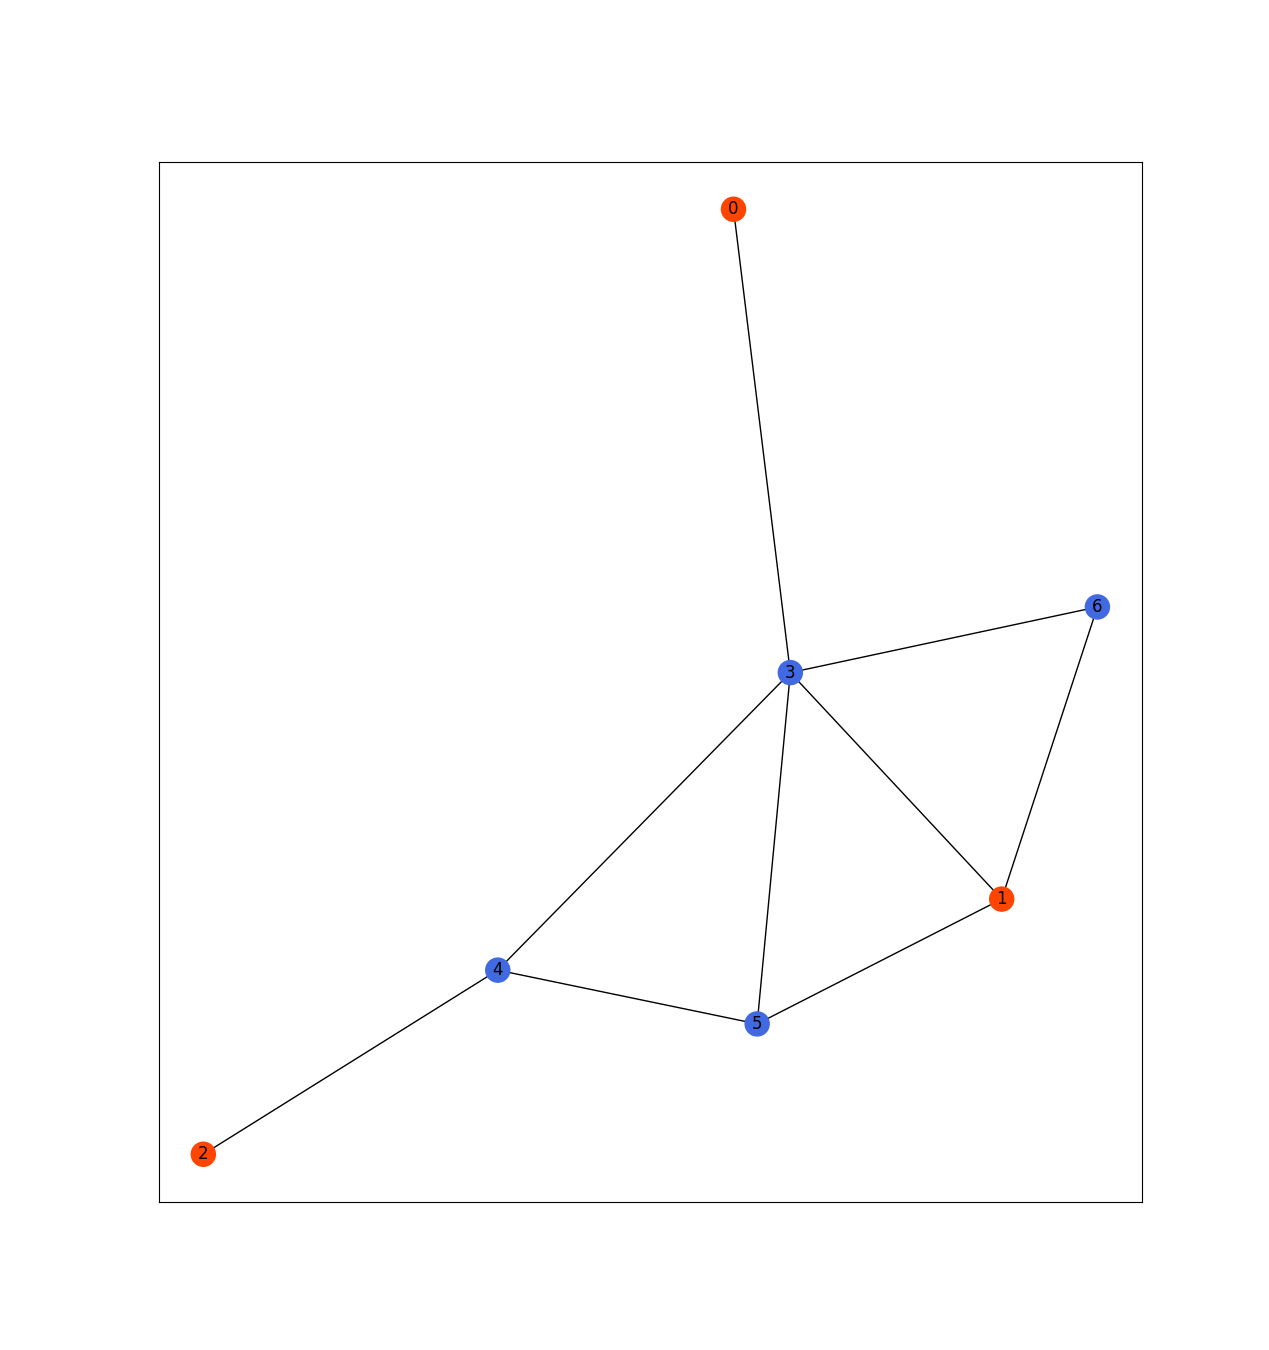
\includegraphics[height=0.7\textheight]{Figure_1.png}
  % \begin{columns}[T] % align columns
  %   \begin{column}{.48\textwidth}
  %   \end{column}%
  %   \hfill%
  %   \begin{column}{.48\textwidth} 
  %   \end{column}%
  % \end{columns}
\end{frame}

\section{Intuitive Approach}
\begin{frame}{Intuitive Approach \trivial}
  \begin{itemize}
    \item Iterate over all vertices
    \item Check if vertex can be in MIS
    \item Complexity: $\mathcal{O}(m)$
    \pause
    \bigskip
    \item Recompute after every update
  \end{itemize} 
\end{frame}

% \section{Types of updates}
\begin{frame}{Types of updates}
  \begin{itemize}
    \item Node removal

    \item Node insertion 
    
    \item Edge removal

    \item Edge insertion

    \bigskip
    \item 1 node might leave \M
    \item up to $\Delta$ might enter \M 
  \end{itemize}
  
\end{frame}

% \section{Amortized Complexity}
% \begin{frame} 
% \end{frame}

\section{Simple Dynamic Algorithm}
\begin{frame}{Simple Dynamic Algorithm \simple}
  \begin{itemize}
    \item Every vertex has counter of neighbors in \M
    \item If counter == 0: vertex can be added 
    \pause
    \medskip
    \item Every node joining/leaving \M\ has to inform $\mathcal{O}(\Delta)$ neighbors
    \medskip
    \item amortized time per update: \OD
    \pause
    \bigskip
    \item Why? \OD\ insertions costing \OD\ each!
    \\
    \pause
    $\rightarrow$ Assign cost of next insertion to removal
  \end{itemize}
  
\end{frame}

\section{Improved Dynamic Algorithm}
\begin{frame}{Improved Dynamic Algorithm}
  \begin{itemize}
    \item Complexity of \simple\ is determined by high degree nodes
    \pause
    \medskip
    \item Idea: differentiate between \textbf{heavy} and \textbf{light} vertices
    \item $v$ is \textbf{light} if: $deg(v) < \Delta_C$
  \end{itemize}
  \begin{enumerate}
    \pause
    \bigskip
    \item \simple\ for light vertices
    \medskip
    \item \trivial\ for heavy vertices
    \begin{itemize}
      \item respect the IS on the light nodes!
    \end{itemize}
  \end{enumerate} 
\end{frame}

\begin{frame}{Improved Dynamic Algorithm}
  \begin{itemize}
    \item $\Delta_C := m^{2/3}$
    \\
    \pause
    $\rightarrow$ New phase if $m \geq 2m_c \lor m \leq m_c/2$

    \pause
    \bigskip
    \item \simple\ takes $\mathcal{O}(m^{2/3})$

    % FIXME: is this correct?
    \item \trivial\ takes $\mathcal{O}(m_H) = \mathcal{O}((\frac{m}{\Delta_C})^2) = \mathcal{O}(m^{2/3})$

    \pause
    \bigskip
    \item overall amortized complexity: $\mathcal{O}(min\{\Delta, m^{2/3}\})$
    \\
    $\rightarrow$ all nodes could be light
  \end{itemize}
\end{frame}

\section{Implicit MIS Algorithm}
\begin{frame}{Relaxed Model}
  \begin{itemize}
    \item The previous algorithms:
    \begin{itemize}
      \item kept explicit copy of MIS
      \item analyzed for amortized complexity
    \end{itemize}
    % Because worst case adjustment complexity is \Omega(n)
    \pause
    \bigskip
    \item Relax requirement to keep explicit copy of MIS
  \end{itemize} 
\end{frame}

\begin{frame}{Implicit MIS \implicit}
  \begin{itemize}
    \item Only maintain an IS not an MIS
    \item Only process removals of nodes
    \medskip
    \pause
    \item Check if $v \in$ \M\ when asked

    \medskip
    \item Worst case complexity $\mathcal{O}(min\{\Delta, \sqrt{m}\})$
  \end{itemize}
\end{frame}

\begin{frame}{Realisation of \implicit}
  \begin{itemize}
    \item Again \textbf{light} and \textbf{heavy} nodes
    \item $\Delta_C := \sqrt{m}$
    \pause
    \medskip
    \item Maintain count for heavy nodes only
    \item Compute status for light nodes when queried

  \end{itemize}
  
\end{frame}

\begin{frame}{Conclusion}
  \begin{itemize}
    \item Code and slides at: \\
          \href{https://www.github.com/thilofischer/dynamic_mis}{github.com/thilofischer/dynamic\_mis}
  \end{itemize}
\end{frame}


\end{document}
